\documentclass[11pt,a4paper]{article}

% shared/macros.tex
% Shared notation for all surface-partition math documents.
% Include with: % shared/macros.tex
% Shared notation for all surface-partition math documents.
% Include with: % shared/macros.tex
% Shared notation for all surface-partition math documents.
% Include with: \input{../shared/macros}

% -------------------------------------------------------------------------
% Packages (include here so each document only needs \input{../shared/macros})
% -------------------------------------------------------------------------
\usepackage{amsmath,amssymb,amsthm}
\usepackage{bm}           % \bm for bold math
\usepackage{mathtools}    % \coloneqq, dcases, etc.
\usepackage{booktabs}     % \toprule etc. in tables
\usepackage{hyperref}
\usepackage{geometry}
\usepackage{microtype}
\usepackage{parskip}
\usepackage{xcolor}
\usepackage{tcolorbox}
\usepackage{enumitem}
\usepackage{float}             % [H] float placement

\geometry{a4paper, margin=2.5cm}

% -------------------------------------------------------------------------
% Theorem-like environments
% -------------------------------------------------------------------------
\theoremstyle{definition}
\newtheorem{defn}{Definition}[section]
\newtheorem{remark}{Remark}[section]

\theoremstyle{plain}
\newtheorem{prop}{Proposition}[section]

% -------------------------------------------------------------------------
% Mesh and geometry
% -------------------------------------------------------------------------
\newcommand{\V}{\mathbf{V}}            % vertex array V[i] in R^dim
\newcommand{\F}{\mathbf{F}}            % face (triangle) array
\newcommand{\vone}[1]{v_{1,#1}}       % first vertex index of VP i
\newcommand{\vtwo}[1]{v_{2,#1}}       % second vertex index of VP i

% -------------------------------------------------------------------------
% Variable points
% -------------------------------------------------------------------------
\newcommand{\lam}{\lambda}             % scalar VP parameter
\newcommand{\Lam}{\boldsymbol{\lambda}}% full parameter vector
\newcommand{\vp}[1]{\mathbf{p}_{#1}}  % 3D position of VP i
\newcommand{\ed}[1]{\mathbf{d}_{#1}}  % edge direction d_i = V[v1_i] - V[v2_i]

% -------------------------------------------------------------------------
% Steiner / triple-point
% -------------------------------------------------------------------------
\newcommand{\Sv}{\mathbf{S}}           % Steiner (Fermat-Torricelli) point
\newcommand{\Ki}{K_{i}}               % projection matrix (I-n_i n_i^T)/r_i
\newcommand{\Mmat}{M}                 % sum of K_i matrices at a triple point

% -------------------------------------------------------------------------
% Normals and unit vectors
% -------------------------------------------------------------------------
\newcommand{\nhat}{\hat{\mathbf{n}}}  % unit normal to a triangle
\newcommand{\Dhat}{\hat{\boldsymbol{\Delta}}}  % unit segment direction

% -------------------------------------------------------------------------
% Operations
% -------------------------------------------------------------------------
\newcommand{\norm}[1]{\left\|#1\right\|}
\newcommand{\abs}[1]{\left|#1\right|}
\newcommand{\ip}[2]{\langle #1,\, #2 \rangle}

% Projection perpendicular to a unit vector \uhat
\newcommand{\Proj}[1]{\bigl(\mathbf{I} - #1 #1^\top\bigr)}

% argmax operator (winner-take-all assignment in Phase 1 documents)
\DeclareMathOperator*{\argmax}{arg\,max}
\DeclareMathOperator*{\argmin}{arg\,min}

% -------------------------------------------------------------------------
% Calculus shorthands
% -------------------------------------------------------------------------
\newcommand{\pd}[2]{\dfrac{\partial #1}{\partial #2}}
\newcommand{\pdd}[3]{\dfrac{\partial^2 #1}{\partial #2\,\partial #3}}
\newcommand{\grad}{\nabla}
\newcommand{\Hess}[1]{\nabla^2 #1}

% -------------------------------------------------------------------------
% Optimization problem objects
% -------------------------------------------------------------------------
\newcommand{\Preg}{P_{\mathrm{reg}}}  % regular perimeter
\newcommand{\Pst}{P_{\mathrm{st}}}   % Steiner perimeter
\newcommand{\Areg}{A^{\mathrm{reg}}} % regular cell area
\newcommand{\Ast}{A^{\mathrm{st}}}   % Steiner area contribution
\newcommand{\Atgt}{\bar{A}}           % target area per cell
\newcommand{\Lagr}{\mathcal{L}}       % Lagrangian
\newcommand{\objfac}{\sigma}          % IPOPT objective scaling factor

% -------------------------------------------------------------------------
% Code cross-references (for "In the code..." callouts)
% -------------------------------------------------------------------------
\newcommand{\code}[1]{\texttt{#1}}
\newcommand{\codefile}[1]{\texttt{\small #1}}

% -------------------------------------------------------------------------
% Threshold dynamics / approach B (10-mbo-auction-dynamics)
% -------------------------------------------------------------------------
\newcommand{\Dlump}{D}                 % lumped mass matrix diag(v)
\newcommand{\Atau}{A_\tau}             % discrete diffusion operator (M + tau K)^{-1} M
\newcommand{\Etau}{E_\tau}             % heat-content (threshold-dynamics) energy
\newcommand{\Rcell}{R_{\mathrm{cell}}} % radius of the equal-area disc sqrt(Abar/pi)
\newcommand{\hmean}{h_{\mathrm{mean}}} % mean edge length
\newcommand{\hmax}{h_{\mathrm{max}}}   % max edge length
\newcommand{\Gt}{G_t}                  % heat kernel at time t
\newcommand{\Ktau}{K^{\mathrm{res}}_\tau} % resolvent (backward-Euler) kernel


% -------------------------------------------------------------------------
% Packages (include here so each document only needs % shared/macros.tex
% Shared notation for all surface-partition math documents.
% Include with: \input{../shared/macros}

% -------------------------------------------------------------------------
% Packages (include here so each document only needs \input{../shared/macros})
% -------------------------------------------------------------------------
\usepackage{amsmath,amssymb,amsthm}
\usepackage{bm}           % \bm for bold math
\usepackage{mathtools}    % \coloneqq, dcases, etc.
\usepackage{booktabs}     % \toprule etc. in tables
\usepackage{hyperref}
\usepackage{geometry}
\usepackage{microtype}
\usepackage{parskip}
\usepackage{xcolor}
\usepackage{tcolorbox}
\usepackage{enumitem}
\usepackage{float}             % [H] float placement

\geometry{a4paper, margin=2.5cm}

% -------------------------------------------------------------------------
% Theorem-like environments
% -------------------------------------------------------------------------
\theoremstyle{definition}
\newtheorem{defn}{Definition}[section]
\newtheorem{remark}{Remark}[section]

\theoremstyle{plain}
\newtheorem{prop}{Proposition}[section]

% -------------------------------------------------------------------------
% Mesh and geometry
% -------------------------------------------------------------------------
\newcommand{\V}{\mathbf{V}}            % vertex array V[i] in R^dim
\newcommand{\F}{\mathbf{F}}            % face (triangle) array
\newcommand{\vone}[1]{v_{1,#1}}       % first vertex index of VP i
\newcommand{\vtwo}[1]{v_{2,#1}}       % second vertex index of VP i

% -------------------------------------------------------------------------
% Variable points
% -------------------------------------------------------------------------
\newcommand{\lam}{\lambda}             % scalar VP parameter
\newcommand{\Lam}{\boldsymbol{\lambda}}% full parameter vector
\newcommand{\vp}[1]{\mathbf{p}_{#1}}  % 3D position of VP i
\newcommand{\ed}[1]{\mathbf{d}_{#1}}  % edge direction d_i = V[v1_i] - V[v2_i]

% -------------------------------------------------------------------------
% Steiner / triple-point
% -------------------------------------------------------------------------
\newcommand{\Sv}{\mathbf{S}}           % Steiner (Fermat-Torricelli) point
\newcommand{\Ki}{K_{i}}               % projection matrix (I-n_i n_i^T)/r_i
\newcommand{\Mmat}{M}                 % sum of K_i matrices at a triple point

% -------------------------------------------------------------------------
% Normals and unit vectors
% -------------------------------------------------------------------------
\newcommand{\nhat}{\hat{\mathbf{n}}}  % unit normal to a triangle
\newcommand{\Dhat}{\hat{\boldsymbol{\Delta}}}  % unit segment direction

% -------------------------------------------------------------------------
% Operations
% -------------------------------------------------------------------------
\newcommand{\norm}[1]{\left\|#1\right\|}
\newcommand{\abs}[1]{\left|#1\right|}
\newcommand{\ip}[2]{\langle #1,\, #2 \rangle}

% Projection perpendicular to a unit vector \uhat
\newcommand{\Proj}[1]{\bigl(\mathbf{I} - #1 #1^\top\bigr)}

% argmax operator (winner-take-all assignment in Phase 1 documents)
\DeclareMathOperator*{\argmax}{arg\,max}
\DeclareMathOperator*{\argmin}{arg\,min}

% -------------------------------------------------------------------------
% Calculus shorthands
% -------------------------------------------------------------------------
\newcommand{\pd}[2]{\dfrac{\partial #1}{\partial #2}}
\newcommand{\pdd}[3]{\dfrac{\partial^2 #1}{\partial #2\,\partial #3}}
\newcommand{\grad}{\nabla}
\newcommand{\Hess}[1]{\nabla^2 #1}

% -------------------------------------------------------------------------
% Optimization problem objects
% -------------------------------------------------------------------------
\newcommand{\Preg}{P_{\mathrm{reg}}}  % regular perimeter
\newcommand{\Pst}{P_{\mathrm{st}}}   % Steiner perimeter
\newcommand{\Areg}{A^{\mathrm{reg}}} % regular cell area
\newcommand{\Ast}{A^{\mathrm{st}}}   % Steiner area contribution
\newcommand{\Atgt}{\bar{A}}           % target area per cell
\newcommand{\Lagr}{\mathcal{L}}       % Lagrangian
\newcommand{\objfac}{\sigma}          % IPOPT objective scaling factor

% -------------------------------------------------------------------------
% Code cross-references (for "In the code..." callouts)
% -------------------------------------------------------------------------
\newcommand{\code}[1]{\texttt{#1}}
\newcommand{\codefile}[1]{\texttt{\small #1}}

% -------------------------------------------------------------------------
% Threshold dynamics / approach B (10-mbo-auction-dynamics)
% -------------------------------------------------------------------------
\newcommand{\Dlump}{D}                 % lumped mass matrix diag(v)
\newcommand{\Atau}{A_\tau}             % discrete diffusion operator (M + tau K)^{-1} M
\newcommand{\Etau}{E_\tau}             % heat-content (threshold-dynamics) energy
\newcommand{\Rcell}{R_{\mathrm{cell}}} % radius of the equal-area disc sqrt(Abar/pi)
\newcommand{\hmean}{h_{\mathrm{mean}}} % mean edge length
\newcommand{\hmax}{h_{\mathrm{max}}}   % max edge length
\newcommand{\Gt}{G_t}                  % heat kernel at time t
\newcommand{\Ktau}{K^{\mathrm{res}}_\tau} % resolvent (backward-Euler) kernel
)
% -------------------------------------------------------------------------
\usepackage{amsmath,amssymb,amsthm}
\usepackage{bm}           % \bm for bold math
\usepackage{mathtools}    % \coloneqq, dcases, etc.
\usepackage{booktabs}     % \toprule etc. in tables
\usepackage{hyperref}
\usepackage{geometry}
\usepackage{microtype}
\usepackage{parskip}
\usepackage{xcolor}
\usepackage{tcolorbox}
\usepackage{enumitem}
\usepackage{float}             % [H] float placement

\geometry{a4paper, margin=2.5cm}

% -------------------------------------------------------------------------
% Theorem-like environments
% -------------------------------------------------------------------------
\theoremstyle{definition}
\newtheorem{defn}{Definition}[section]
\newtheorem{remark}{Remark}[section]

\theoremstyle{plain}
\newtheorem{prop}{Proposition}[section]

% -------------------------------------------------------------------------
% Mesh and geometry
% -------------------------------------------------------------------------
\newcommand{\V}{\mathbf{V}}            % vertex array V[i] in R^dim
\newcommand{\F}{\mathbf{F}}            % face (triangle) array
\newcommand{\vone}[1]{v_{1,#1}}       % first vertex index of VP i
\newcommand{\vtwo}[1]{v_{2,#1}}       % second vertex index of VP i

% -------------------------------------------------------------------------
% Variable points
% -------------------------------------------------------------------------
\newcommand{\lam}{\lambda}             % scalar VP parameter
\newcommand{\Lam}{\boldsymbol{\lambda}}% full parameter vector
\newcommand{\vp}[1]{\mathbf{p}_{#1}}  % 3D position of VP i
\newcommand{\ed}[1]{\mathbf{d}_{#1}}  % edge direction d_i = V[v1_i] - V[v2_i]

% -------------------------------------------------------------------------
% Steiner / triple-point
% -------------------------------------------------------------------------
\newcommand{\Sv}{\mathbf{S}}           % Steiner (Fermat-Torricelli) point
\newcommand{\Ki}{K_{i}}               % projection matrix (I-n_i n_i^T)/r_i
\newcommand{\Mmat}{M}                 % sum of K_i matrices at a triple point

% -------------------------------------------------------------------------
% Normals and unit vectors
% -------------------------------------------------------------------------
\newcommand{\nhat}{\hat{\mathbf{n}}}  % unit normal to a triangle
\newcommand{\Dhat}{\hat{\boldsymbol{\Delta}}}  % unit segment direction

% -------------------------------------------------------------------------
% Operations
% -------------------------------------------------------------------------
\newcommand{\norm}[1]{\left\|#1\right\|}
\newcommand{\abs}[1]{\left|#1\right|}
\newcommand{\ip}[2]{\langle #1,\, #2 \rangle}

% Projection perpendicular to a unit vector \uhat
\newcommand{\Proj}[1]{\bigl(\mathbf{I} - #1 #1^\top\bigr)}

% argmax operator (winner-take-all assignment in Phase 1 documents)
\DeclareMathOperator*{\argmax}{arg\,max}
\DeclareMathOperator*{\argmin}{arg\,min}

% -------------------------------------------------------------------------
% Calculus shorthands
% -------------------------------------------------------------------------
\newcommand{\pd}[2]{\dfrac{\partial #1}{\partial #2}}
\newcommand{\pdd}[3]{\dfrac{\partial^2 #1}{\partial #2\,\partial #3}}
\newcommand{\grad}{\nabla}
\newcommand{\Hess}[1]{\nabla^2 #1}

% -------------------------------------------------------------------------
% Optimization problem objects
% -------------------------------------------------------------------------
\newcommand{\Preg}{P_{\mathrm{reg}}}  % regular perimeter
\newcommand{\Pst}{P_{\mathrm{st}}}   % Steiner perimeter
\newcommand{\Areg}{A^{\mathrm{reg}}} % regular cell area
\newcommand{\Ast}{A^{\mathrm{st}}}   % Steiner area contribution
\newcommand{\Atgt}{\bar{A}}           % target area per cell
\newcommand{\Lagr}{\mathcal{L}}       % Lagrangian
\newcommand{\objfac}{\sigma}          % IPOPT objective scaling factor

% -------------------------------------------------------------------------
% Code cross-references (for "In the code..." callouts)
% -------------------------------------------------------------------------
\newcommand{\code}[1]{\texttt{#1}}
\newcommand{\codefile}[1]{\texttt{\small #1}}

% -------------------------------------------------------------------------
% Threshold dynamics / approach B (10-mbo-auction-dynamics)
% -------------------------------------------------------------------------
\newcommand{\Dlump}{D}                 % lumped mass matrix diag(v)
\newcommand{\Atau}{A_\tau}             % discrete diffusion operator (M + tau K)^{-1} M
\newcommand{\Etau}{E_\tau}             % heat-content (threshold-dynamics) energy
\newcommand{\Rcell}{R_{\mathrm{cell}}} % radius of the equal-area disc sqrt(Abar/pi)
\newcommand{\hmean}{h_{\mathrm{mean}}} % mean edge length
\newcommand{\hmax}{h_{\mathrm{max}}}   % max edge length
\newcommand{\Gt}{G_t}                  % heat kernel at time t
\newcommand{\Ktau}{K^{\mathrm{res}}_\tau} % resolvent (backward-Euler) kernel


% -------------------------------------------------------------------------
% Packages (include here so each document only needs % shared/macros.tex
% Shared notation for all surface-partition math documents.
% Include with: % shared/macros.tex
% Shared notation for all surface-partition math documents.
% Include with: \input{../shared/macros}

% -------------------------------------------------------------------------
% Packages (include here so each document only needs \input{../shared/macros})
% -------------------------------------------------------------------------
\usepackage{amsmath,amssymb,amsthm}
\usepackage{bm}           % \bm for bold math
\usepackage{mathtools}    % \coloneqq, dcases, etc.
\usepackage{booktabs}     % \toprule etc. in tables
\usepackage{hyperref}
\usepackage{geometry}
\usepackage{microtype}
\usepackage{parskip}
\usepackage{xcolor}
\usepackage{tcolorbox}
\usepackage{enumitem}
\usepackage{float}             % [H] float placement

\geometry{a4paper, margin=2.5cm}

% -------------------------------------------------------------------------
% Theorem-like environments
% -------------------------------------------------------------------------
\theoremstyle{definition}
\newtheorem{defn}{Definition}[section]
\newtheorem{remark}{Remark}[section]

\theoremstyle{plain}
\newtheorem{prop}{Proposition}[section]

% -------------------------------------------------------------------------
% Mesh and geometry
% -------------------------------------------------------------------------
\newcommand{\V}{\mathbf{V}}            % vertex array V[i] in R^dim
\newcommand{\F}{\mathbf{F}}            % face (triangle) array
\newcommand{\vone}[1]{v_{1,#1}}       % first vertex index of VP i
\newcommand{\vtwo}[1]{v_{2,#1}}       % second vertex index of VP i

% -------------------------------------------------------------------------
% Variable points
% -------------------------------------------------------------------------
\newcommand{\lam}{\lambda}             % scalar VP parameter
\newcommand{\Lam}{\boldsymbol{\lambda}}% full parameter vector
\newcommand{\vp}[1]{\mathbf{p}_{#1}}  % 3D position of VP i
\newcommand{\ed}[1]{\mathbf{d}_{#1}}  % edge direction d_i = V[v1_i] - V[v2_i]

% -------------------------------------------------------------------------
% Steiner / triple-point
% -------------------------------------------------------------------------
\newcommand{\Sv}{\mathbf{S}}           % Steiner (Fermat-Torricelli) point
\newcommand{\Ki}{K_{i}}               % projection matrix (I-n_i n_i^T)/r_i
\newcommand{\Mmat}{M}                 % sum of K_i matrices at a triple point

% -------------------------------------------------------------------------
% Normals and unit vectors
% -------------------------------------------------------------------------
\newcommand{\nhat}{\hat{\mathbf{n}}}  % unit normal to a triangle
\newcommand{\Dhat}{\hat{\boldsymbol{\Delta}}}  % unit segment direction

% -------------------------------------------------------------------------
% Operations
% -------------------------------------------------------------------------
\newcommand{\norm}[1]{\left\|#1\right\|}
\newcommand{\abs}[1]{\left|#1\right|}
\newcommand{\ip}[2]{\langle #1,\, #2 \rangle}

% Projection perpendicular to a unit vector \uhat
\newcommand{\Proj}[1]{\bigl(\mathbf{I} - #1 #1^\top\bigr)}

% argmax operator (winner-take-all assignment in Phase 1 documents)
\DeclareMathOperator*{\argmax}{arg\,max}
\DeclareMathOperator*{\argmin}{arg\,min}

% -------------------------------------------------------------------------
% Calculus shorthands
% -------------------------------------------------------------------------
\newcommand{\pd}[2]{\dfrac{\partial #1}{\partial #2}}
\newcommand{\pdd}[3]{\dfrac{\partial^2 #1}{\partial #2\,\partial #3}}
\newcommand{\grad}{\nabla}
\newcommand{\Hess}[1]{\nabla^2 #1}

% -------------------------------------------------------------------------
% Optimization problem objects
% -------------------------------------------------------------------------
\newcommand{\Preg}{P_{\mathrm{reg}}}  % regular perimeter
\newcommand{\Pst}{P_{\mathrm{st}}}   % Steiner perimeter
\newcommand{\Areg}{A^{\mathrm{reg}}} % regular cell area
\newcommand{\Ast}{A^{\mathrm{st}}}   % Steiner area contribution
\newcommand{\Atgt}{\bar{A}}           % target area per cell
\newcommand{\Lagr}{\mathcal{L}}       % Lagrangian
\newcommand{\objfac}{\sigma}          % IPOPT objective scaling factor

% -------------------------------------------------------------------------
% Code cross-references (for "In the code..." callouts)
% -------------------------------------------------------------------------
\newcommand{\code}[1]{\texttt{#1}}
\newcommand{\codefile}[1]{\texttt{\small #1}}

% -------------------------------------------------------------------------
% Threshold dynamics / approach B (10-mbo-auction-dynamics)
% -------------------------------------------------------------------------
\newcommand{\Dlump}{D}                 % lumped mass matrix diag(v)
\newcommand{\Atau}{A_\tau}             % discrete diffusion operator (M + tau K)^{-1} M
\newcommand{\Etau}{E_\tau}             % heat-content (threshold-dynamics) energy
\newcommand{\Rcell}{R_{\mathrm{cell}}} % radius of the equal-area disc sqrt(Abar/pi)
\newcommand{\hmean}{h_{\mathrm{mean}}} % mean edge length
\newcommand{\hmax}{h_{\mathrm{max}}}   % max edge length
\newcommand{\Gt}{G_t}                  % heat kernel at time t
\newcommand{\Ktau}{K^{\mathrm{res}}_\tau} % resolvent (backward-Euler) kernel


% -------------------------------------------------------------------------
% Packages (include here so each document only needs % shared/macros.tex
% Shared notation for all surface-partition math documents.
% Include with: \input{../shared/macros}

% -------------------------------------------------------------------------
% Packages (include here so each document only needs \input{../shared/macros})
% -------------------------------------------------------------------------
\usepackage{amsmath,amssymb,amsthm}
\usepackage{bm}           % \bm for bold math
\usepackage{mathtools}    % \coloneqq, dcases, etc.
\usepackage{booktabs}     % \toprule etc. in tables
\usepackage{hyperref}
\usepackage{geometry}
\usepackage{microtype}
\usepackage{parskip}
\usepackage{xcolor}
\usepackage{tcolorbox}
\usepackage{enumitem}
\usepackage{float}             % [H] float placement

\geometry{a4paper, margin=2.5cm}

% -------------------------------------------------------------------------
% Theorem-like environments
% -------------------------------------------------------------------------
\theoremstyle{definition}
\newtheorem{defn}{Definition}[section]
\newtheorem{remark}{Remark}[section]

\theoremstyle{plain}
\newtheorem{prop}{Proposition}[section]

% -------------------------------------------------------------------------
% Mesh and geometry
% -------------------------------------------------------------------------
\newcommand{\V}{\mathbf{V}}            % vertex array V[i] in R^dim
\newcommand{\F}{\mathbf{F}}            % face (triangle) array
\newcommand{\vone}[1]{v_{1,#1}}       % first vertex index of VP i
\newcommand{\vtwo}[1]{v_{2,#1}}       % second vertex index of VP i

% -------------------------------------------------------------------------
% Variable points
% -------------------------------------------------------------------------
\newcommand{\lam}{\lambda}             % scalar VP parameter
\newcommand{\Lam}{\boldsymbol{\lambda}}% full parameter vector
\newcommand{\vp}[1]{\mathbf{p}_{#1}}  % 3D position of VP i
\newcommand{\ed}[1]{\mathbf{d}_{#1}}  % edge direction d_i = V[v1_i] - V[v2_i]

% -------------------------------------------------------------------------
% Steiner / triple-point
% -------------------------------------------------------------------------
\newcommand{\Sv}{\mathbf{S}}           % Steiner (Fermat-Torricelli) point
\newcommand{\Ki}{K_{i}}               % projection matrix (I-n_i n_i^T)/r_i
\newcommand{\Mmat}{M}                 % sum of K_i matrices at a triple point

% -------------------------------------------------------------------------
% Normals and unit vectors
% -------------------------------------------------------------------------
\newcommand{\nhat}{\hat{\mathbf{n}}}  % unit normal to a triangle
\newcommand{\Dhat}{\hat{\boldsymbol{\Delta}}}  % unit segment direction

% -------------------------------------------------------------------------
% Operations
% -------------------------------------------------------------------------
\newcommand{\norm}[1]{\left\|#1\right\|}
\newcommand{\abs}[1]{\left|#1\right|}
\newcommand{\ip}[2]{\langle #1,\, #2 \rangle}

% Projection perpendicular to a unit vector \uhat
\newcommand{\Proj}[1]{\bigl(\mathbf{I} - #1 #1^\top\bigr)}

% argmax operator (winner-take-all assignment in Phase 1 documents)
\DeclareMathOperator*{\argmax}{arg\,max}
\DeclareMathOperator*{\argmin}{arg\,min}

% -------------------------------------------------------------------------
% Calculus shorthands
% -------------------------------------------------------------------------
\newcommand{\pd}[2]{\dfrac{\partial #1}{\partial #2}}
\newcommand{\pdd}[3]{\dfrac{\partial^2 #1}{\partial #2\,\partial #3}}
\newcommand{\grad}{\nabla}
\newcommand{\Hess}[1]{\nabla^2 #1}

% -------------------------------------------------------------------------
% Optimization problem objects
% -------------------------------------------------------------------------
\newcommand{\Preg}{P_{\mathrm{reg}}}  % regular perimeter
\newcommand{\Pst}{P_{\mathrm{st}}}   % Steiner perimeter
\newcommand{\Areg}{A^{\mathrm{reg}}} % regular cell area
\newcommand{\Ast}{A^{\mathrm{st}}}   % Steiner area contribution
\newcommand{\Atgt}{\bar{A}}           % target area per cell
\newcommand{\Lagr}{\mathcal{L}}       % Lagrangian
\newcommand{\objfac}{\sigma}          % IPOPT objective scaling factor

% -------------------------------------------------------------------------
% Code cross-references (for "In the code..." callouts)
% -------------------------------------------------------------------------
\newcommand{\code}[1]{\texttt{#1}}
\newcommand{\codefile}[1]{\texttt{\small #1}}

% -------------------------------------------------------------------------
% Threshold dynamics / approach B (10-mbo-auction-dynamics)
% -------------------------------------------------------------------------
\newcommand{\Dlump}{D}                 % lumped mass matrix diag(v)
\newcommand{\Atau}{A_\tau}             % discrete diffusion operator (M + tau K)^{-1} M
\newcommand{\Etau}{E_\tau}             % heat-content (threshold-dynamics) energy
\newcommand{\Rcell}{R_{\mathrm{cell}}} % radius of the equal-area disc sqrt(Abar/pi)
\newcommand{\hmean}{h_{\mathrm{mean}}} % mean edge length
\newcommand{\hmax}{h_{\mathrm{max}}}   % max edge length
\newcommand{\Gt}{G_t}                  % heat kernel at time t
\newcommand{\Ktau}{K^{\mathrm{res}}_\tau} % resolvent (backward-Euler) kernel
)
% -------------------------------------------------------------------------
\usepackage{amsmath,amssymb,amsthm}
\usepackage{bm}           % \bm for bold math
\usepackage{mathtools}    % \coloneqq, dcases, etc.
\usepackage{booktabs}     % \toprule etc. in tables
\usepackage{hyperref}
\usepackage{geometry}
\usepackage{microtype}
\usepackage{parskip}
\usepackage{xcolor}
\usepackage{tcolorbox}
\usepackage{enumitem}
\usepackage{float}             % [H] float placement

\geometry{a4paper, margin=2.5cm}

% -------------------------------------------------------------------------
% Theorem-like environments
% -------------------------------------------------------------------------
\theoremstyle{definition}
\newtheorem{defn}{Definition}[section]
\newtheorem{remark}{Remark}[section]

\theoremstyle{plain}
\newtheorem{prop}{Proposition}[section]

% -------------------------------------------------------------------------
% Mesh and geometry
% -------------------------------------------------------------------------
\newcommand{\V}{\mathbf{V}}            % vertex array V[i] in R^dim
\newcommand{\F}{\mathbf{F}}            % face (triangle) array
\newcommand{\vone}[1]{v_{1,#1}}       % first vertex index of VP i
\newcommand{\vtwo}[1]{v_{2,#1}}       % second vertex index of VP i

% -------------------------------------------------------------------------
% Variable points
% -------------------------------------------------------------------------
\newcommand{\lam}{\lambda}             % scalar VP parameter
\newcommand{\Lam}{\boldsymbol{\lambda}}% full parameter vector
\newcommand{\vp}[1]{\mathbf{p}_{#1}}  % 3D position of VP i
\newcommand{\ed}[1]{\mathbf{d}_{#1}}  % edge direction d_i = V[v1_i] - V[v2_i]

% -------------------------------------------------------------------------
% Steiner / triple-point
% -------------------------------------------------------------------------
\newcommand{\Sv}{\mathbf{S}}           % Steiner (Fermat-Torricelli) point
\newcommand{\Ki}{K_{i}}               % projection matrix (I-n_i n_i^T)/r_i
\newcommand{\Mmat}{M}                 % sum of K_i matrices at a triple point

% -------------------------------------------------------------------------
% Normals and unit vectors
% -------------------------------------------------------------------------
\newcommand{\nhat}{\hat{\mathbf{n}}}  % unit normal to a triangle
\newcommand{\Dhat}{\hat{\boldsymbol{\Delta}}}  % unit segment direction

% -------------------------------------------------------------------------
% Operations
% -------------------------------------------------------------------------
\newcommand{\norm}[1]{\left\|#1\right\|}
\newcommand{\abs}[1]{\left|#1\right|}
\newcommand{\ip}[2]{\langle #1,\, #2 \rangle}

% Projection perpendicular to a unit vector \uhat
\newcommand{\Proj}[1]{\bigl(\mathbf{I} - #1 #1^\top\bigr)}

% argmax operator (winner-take-all assignment in Phase 1 documents)
\DeclareMathOperator*{\argmax}{arg\,max}
\DeclareMathOperator*{\argmin}{arg\,min}

% -------------------------------------------------------------------------
% Calculus shorthands
% -------------------------------------------------------------------------
\newcommand{\pd}[2]{\dfrac{\partial #1}{\partial #2}}
\newcommand{\pdd}[3]{\dfrac{\partial^2 #1}{\partial #2\,\partial #3}}
\newcommand{\grad}{\nabla}
\newcommand{\Hess}[1]{\nabla^2 #1}

% -------------------------------------------------------------------------
% Optimization problem objects
% -------------------------------------------------------------------------
\newcommand{\Preg}{P_{\mathrm{reg}}}  % regular perimeter
\newcommand{\Pst}{P_{\mathrm{st}}}   % Steiner perimeter
\newcommand{\Areg}{A^{\mathrm{reg}}} % regular cell area
\newcommand{\Ast}{A^{\mathrm{st}}}   % Steiner area contribution
\newcommand{\Atgt}{\bar{A}}           % target area per cell
\newcommand{\Lagr}{\mathcal{L}}       % Lagrangian
\newcommand{\objfac}{\sigma}          % IPOPT objective scaling factor

% -------------------------------------------------------------------------
% Code cross-references (for "In the code..." callouts)
% -------------------------------------------------------------------------
\newcommand{\code}[1]{\texttt{#1}}
\newcommand{\codefile}[1]{\texttt{\small #1}}

% -------------------------------------------------------------------------
% Threshold dynamics / approach B (10-mbo-auction-dynamics)
% -------------------------------------------------------------------------
\newcommand{\Dlump}{D}                 % lumped mass matrix diag(v)
\newcommand{\Atau}{A_\tau}             % discrete diffusion operator (M + tau K)^{-1} M
\newcommand{\Etau}{E_\tau}             % heat-content (threshold-dynamics) energy
\newcommand{\Rcell}{R_{\mathrm{cell}}} % radius of the equal-area disc sqrt(Abar/pi)
\newcommand{\hmean}{h_{\mathrm{mean}}} % mean edge length
\newcommand{\hmax}{h_{\mathrm{max}}}   % max edge length
\newcommand{\Gt}{G_t}                  % heat kernel at time t
\newcommand{\Ktau}{K^{\mathrm{res}}_\tau} % resolvent (backward-Euler) kernel
)
% -------------------------------------------------------------------------
\usepackage{amsmath,amssymb,amsthm}
\usepackage{bm}           % \bm for bold math
\usepackage{mathtools}    % \coloneqq, dcases, etc.
\usepackage{booktabs}     % \toprule etc. in tables
\usepackage{hyperref}
\usepackage{geometry}
\usepackage{microtype}
\usepackage{parskip}
\usepackage{xcolor}
\usepackage{tcolorbox}
\usepackage{enumitem}
\usepackage{float}             % [H] float placement

\geometry{a4paper, margin=2.5cm}

% -------------------------------------------------------------------------
% Theorem-like environments
% -------------------------------------------------------------------------
\theoremstyle{definition}
\newtheorem{defn}{Definition}[section]
\newtheorem{remark}{Remark}[section]

\theoremstyle{plain}
\newtheorem{prop}{Proposition}[section]

% -------------------------------------------------------------------------
% Mesh and geometry
% -------------------------------------------------------------------------
\newcommand{\V}{\mathbf{V}}            % vertex array V[i] in R^dim
\newcommand{\F}{\mathbf{F}}            % face (triangle) array
\newcommand{\vone}[1]{v_{1,#1}}       % first vertex index of VP i
\newcommand{\vtwo}[1]{v_{2,#1}}       % second vertex index of VP i

% -------------------------------------------------------------------------
% Variable points
% -------------------------------------------------------------------------
\newcommand{\lam}{\lambda}             % scalar VP parameter
\newcommand{\Lam}{\boldsymbol{\lambda}}% full parameter vector
\newcommand{\vp}[1]{\mathbf{p}_{#1}}  % 3D position of VP i
\newcommand{\ed}[1]{\mathbf{d}_{#1}}  % edge direction d_i = V[v1_i] - V[v2_i]

% -------------------------------------------------------------------------
% Steiner / triple-point
% -------------------------------------------------------------------------
\newcommand{\Sv}{\mathbf{S}}           % Steiner (Fermat-Torricelli) point
\newcommand{\Ki}{K_{i}}               % projection matrix (I-n_i n_i^T)/r_i
\newcommand{\Mmat}{M}                 % sum of K_i matrices at a triple point

% -------------------------------------------------------------------------
% Normals and unit vectors
% -------------------------------------------------------------------------
\newcommand{\nhat}{\hat{\mathbf{n}}}  % unit normal to a triangle
\newcommand{\Dhat}{\hat{\boldsymbol{\Delta}}}  % unit segment direction

% -------------------------------------------------------------------------
% Operations
% -------------------------------------------------------------------------
\newcommand{\norm}[1]{\left\|#1\right\|}
\newcommand{\abs}[1]{\left|#1\right|}
\newcommand{\ip}[2]{\langle #1,\, #2 \rangle}

% Projection perpendicular to a unit vector \uhat
\newcommand{\Proj}[1]{\bigl(\mathbf{I} - #1 #1^\top\bigr)}

% argmax operator (winner-take-all assignment in Phase 1 documents)
\DeclareMathOperator*{\argmax}{arg\,max}
\DeclareMathOperator*{\argmin}{arg\,min}

% -------------------------------------------------------------------------
% Calculus shorthands
% -------------------------------------------------------------------------
\newcommand{\pd}[2]{\dfrac{\partial #1}{\partial #2}}
\newcommand{\pdd}[3]{\dfrac{\partial^2 #1}{\partial #2\,\partial #3}}
\newcommand{\grad}{\nabla}
\newcommand{\Hess}[1]{\nabla^2 #1}

% -------------------------------------------------------------------------
% Optimization problem objects
% -------------------------------------------------------------------------
\newcommand{\Preg}{P_{\mathrm{reg}}}  % regular perimeter
\newcommand{\Pst}{P_{\mathrm{st}}}   % Steiner perimeter
\newcommand{\Areg}{A^{\mathrm{reg}}} % regular cell area
\newcommand{\Ast}{A^{\mathrm{st}}}   % Steiner area contribution
\newcommand{\Atgt}{\bar{A}}           % target area per cell
\newcommand{\Lagr}{\mathcal{L}}       % Lagrangian
\newcommand{\objfac}{\sigma}          % IPOPT objective scaling factor

% -------------------------------------------------------------------------
% Code cross-references (for "In the code..." callouts)
% -------------------------------------------------------------------------
\newcommand{\code}[1]{\texttt{#1}}
\newcommand{\codefile}[1]{\texttt{\small #1}}

% -------------------------------------------------------------------------
% Threshold dynamics / approach B (10-mbo-auction-dynamics)
% -------------------------------------------------------------------------
\newcommand{\Dlump}{D}                 % lumped mass matrix diag(v)
\newcommand{\Atau}{A_\tau}             % discrete diffusion operator (M + tau K)^{-1} M
\newcommand{\Etau}{E_\tau}             % heat-content (threshold-dynamics) energy
\newcommand{\Rcell}{R_{\mathrm{cell}}} % radius of the equal-area disc sqrt(Abar/pi)
\newcommand{\hmean}{h_{\mathrm{mean}}} % mean edge length
\newcommand{\hmax}{h_{\mathrm{max}}}   % max edge length
\newcommand{\Gt}{G_t}                  % heat kernel at time t
\newcommand{\Ktau}{K^{\mathrm{res}}_\tau} % resolvent (backward-Euler) kernel
   % shared notation (reused from docs/math/)
\usepackage{graphicx}

\hypersetup{
  colorlinks = true,
  linkcolor  = blue!60!black,
  citecolor  = green!50!black,
  urlcolor   = blue!60!black,
  pdftitle   = {Territory-aware Phase 1: high-N validity validation},
  pdfauthor  = {surface-partition project}
}

\title{\textbf{Territory-Aware Phase~1: Validating the Winner-Take-All Balance
  Term at High \(N\)}\\[0.5em]
  \large On the bad seed that was immune to raising \(\lambda\), the balance term
  drives the entrenched runt from \(-34\%\) to \emph{zero} imbalanced cells --- but
  the discrete-area trim removes the energy plateau, so no level triggers mesh
  refinement, and the coarse level is shown to be resolution-floor-limited}
\author{}
\date{July 2026}

\begin{document}
\maketitle

% ---------------------------------------------------------------------
% STATUS BANNER
% ---------------------------------------------------------------------
\begin{tcolorbox}[colback=green!5!white, colframe=green!55!black,
                  title={Status --- measured (partial: the finest level was
                  interrupted; confirmation is solid through level~1)},
                  fontupper=\small]
This report \textbf{confirms} the Stage-6 hypothesis of the territory-aware
implementation plan (retired; git commit \code{14e0518}): on the
\emph{bad} seed and \(\lambda\) that produced two entrenched \(-34\%\) runts under
the original energy, enabling the winner-take-all balance term drives the partition
to \(0\) imbalanced cells (worst \(\approx 2\%\)), holding through a mesh transition.
It also records two diagnoses of \emph{why the run was slow}: (i) the discrete-area
trim's periodic retargeting removes the energy plateau, so no level fires the mesh
refinement trigger --- every level runs to the iteration cap; and (ii) the coarsest
level is resolution-floor-limited (worst deviation floors at \(\approx 10\%\), above
the \(5\%\) gate), so refinement is \emph{necessary}, not merely faster. Numbers are
independently recomputed from the run's trace snapshots. \textbf{Partial:} the run
died mid-level-2 (host interruption), so the formal finest-level completion gate was
not reached; the confirmation rests on level~1's completed cap and a level-2
mid-snapshot.
\end{tcolorbox}

% ---------------------------------------------------------------------
% ADDENDUM WARNING BANNER (2026-08-03)
% ---------------------------------------------------------------------
\begin{tcolorbox}[colback=red!5!white, colframe=red!60!black,
                  title={Addendum 2026-08-03 --- Result~1 is confirmed only on
                  \emph{area}; the term causes a \emph{connectivity} regression},
                  fontupper=\small]
The July conclusion ``the balance term works'' is measured and stands \textbf{for
the quantity it measured} --- discrete-area imbalance. It did not test
\emph{connectivity}. A later run shows the machinery drives area to target by
handing cells \textbf{disconnected} territory: \(14/200\) fragmented cells, against
\(0\) for the matched term-OFF control at the same seed, \(\lambda\), and mesh.
Together with a wall-clock cost that made a 5-level \(N{=}200\) ladder
unaffordable, this makes the term a \emph{net regression} at \(N{=}200\), where the
original energy already produced a valid finalised partition. See
\S\ref{sec:addendum}. Conclusion~1 of \S\ref{sec:conclusions} must be read with
that qualification.

\medskip
\textbf{Outcome (2026-08-10): the machinery was removed from \code{main}.} The
flags this report exercises (\code{wta\_balance\_enabled},
\code{wta\_trim\_enabled}, \code{pgd\_reduced\_gradient}, \code{wta\_schedule})
\emph{no longer exist} --- reproducing these runs requires checking out commit
\code{14e0518}. The validity gap they targeted is instead closed at extraction by
the balanced readout (\codefile{src/partition/balanced\_readout.py}); see
\codefile{docs/reference/winner\_take\_all\_partition\_gap.md} \S4b and \S9b.
\end{tcolorbox}

% ---------------------------------------------------------------------
% PROVENANCE --- mandatory (docs/experiments/README.md)
% ---------------------------------------------------------------------
\begin{tcolorbox}[colback=gray!4!white, colframe=gray!50!black,
                  title={Provenance}, fontupper=\small]
\begin{tabular}{@{}l@{\hspace{1.5em}}p{0.66\linewidth}@{}}
Date            & 2026-07-20 (analysis of the run of 2026-07-17\,\ldots\,07-19) \\[3pt]
Surface         & torus \(T(R{=}1.0,\ r{=}0.6)\), \(N{=}200\), seed \(84172851\),
                  \(\lambda{=}9\), 3 levels, \code{init\_method: seeded} \\[3pt]
Branch          & \code{feat/phase1-territory-aware-relaxation} \\[3pt]
Source run      & \textbf{territory:} \code{run\_20260717\_102306}, config
                  \codefile{parameters/torus\_200part\_coarse\_seeded\_lam9\_territory\_test.yaml}
                  (\code{wta\_balance\_enabled} \(\gamma{=}7.0\), \(p{=}2\);
                  \code{wta\_trim\_enabled} period 200, damping 0.5, clamp 0.20;
                  \code{pgd\_reduced\_gradient} 8 dual sweeps). \textbf{Control:}
                  \code{run\_20260712\_224424} (same seed/\(\lambda\), original
                  energy, no flags). \\[3pt]
Producing script& \codefile{make\_figures.py} (beside this report; trajectory arrays
                  are the extracted measurement --- see its header) \\[3pt]
Method inputs   & per-level trace snapshots \code{traces/*\_level\{0,1,2\}\_internal\_data.hdf5}
                  (density field \(x\) every 500 iters); the run's \code{relaxation.log} \\[3pt]
Versions        & Python 3.12.13, numpy 2.4.4, scipy 1.17.1, matplotlib 3.10.8,
                  h5py 3.16.0 \\[3pt]
Anchor          & control worst-cell deviation \(=-34.2\%\) (\(2\) imbalanced);
                  territory level-1 end \(=0\) imbalanced, worst \(\pm2.1\%\)
                  (recomputed, matching \code{detect\_area\_imbalance}) \\
\end{tabular}
\end{tcolorbox}

\section{Question}
Phase~1 pins equal area on the \emph{continuous} density field, but the deliverable is
the \emph{argmax} (winner-take-all) partition; at high \(N\) the discrete areas drift,
producing ``runt'' cells that make the Phase-2 equal-area constraint infeasible
(\codefile{docs/reference/winner\_take\_all\_partition\_gap.md}). The territory-aware
term (\codefile{docs/math/07-phase1-wta-balance/}) adds a penalty on the discrete-area
imbalance plus a periodic trim that retargets the projection toward exact discrete
equality. \textbf{Does it fix an entrenched runt on a seed and \(\lambda\) known to be
immune to raising \(\lambda\)} --- the ``anti-lottery'' property N\(=\)1000 needs?

\section{Method}
For each saved snapshot of the density \(x\in\mathbb{R}^{V\times N}\), we rebuild that level's
torus mesh (\code{TorusMeshProvider}), take the winner-take-all label
\(w_i=\argmax_k x_{ik}\), assign each vertex its lumped mass \(v_i\), and form the
discrete cell area \(A_k=\sum_{i:\,w_i=k} v_i\). The relative deviation is
\((A_k-\bar A)/\bar A\) with \(\bar A=\sum_i v_i/N\); a cell is \emph{imbalanced} if
\(|\text{dev}|>5\%\). This is exactly the \code{detect\_area\_imbalance} computation.
All numbers below are recomputed directly from the trace snapshots.

\section{Result 1 --- the mechanism works on the bad seed}
The control (original energy, same seed/\(\lambda\)) ends with worst-cell deviation
\(-34.2\%\) and 2 imbalanced cells. With the territory flags on, the balance improves
monotonically across levels to \(\mathbf{0}\) \textbf{imbalanced cells} (worst
\(\pm2.1\%\)) by the end of level~1, and level~2 inherits and holds it
(Table~\ref{tab:levels}, Fig.~\ref{fig:levels}). No cell dies.

\begin{table}[h]\centering\small
\caption{Winner-take-all discrete-area imbalance, recomputed per level.}
\label{tab:levels}
\begin{tabular}{@{}llrr@{}}
\hline
Level (verts/cell) & snapshot & worst dev & \(n_{\text{imb}}\) \(({>}5\%)\) \\
\hline
Level 0 (48)  & iter 0        & \(-30.3\%/{+}54.0\%\) & 149 \\
Level 0 (48)  & iter 29\,999 (cap) & \(-10.1\%/{+}7.0\%\)  & 4 \\
Level 1 (124) & iter 0 (post-interp) & \(-17.9\%/{+}14.5\%\) & 51 \\
Level 1 (124) & iter 29\,999 (cap) & \(\mathbf{-2.1\%/{+}2.1\%}\) & \(\mathbf{0}\) \\
Level 2 (237) & iter 0 (post-interp) & \(-4.3\%/{+}4.6\%\) & 0 \\
Level 2 (237) & iter 7\,500 (died) & \(-1.5\%/{+}2.4\%\) & 0 \\
\hline
\textit{Control} & final & \(\mathbf{-34.2\%}\) & \(\mathbf{2}\) \\
\hline
\end{tabular}
\end{table}

\begin{figure}[h]\centering
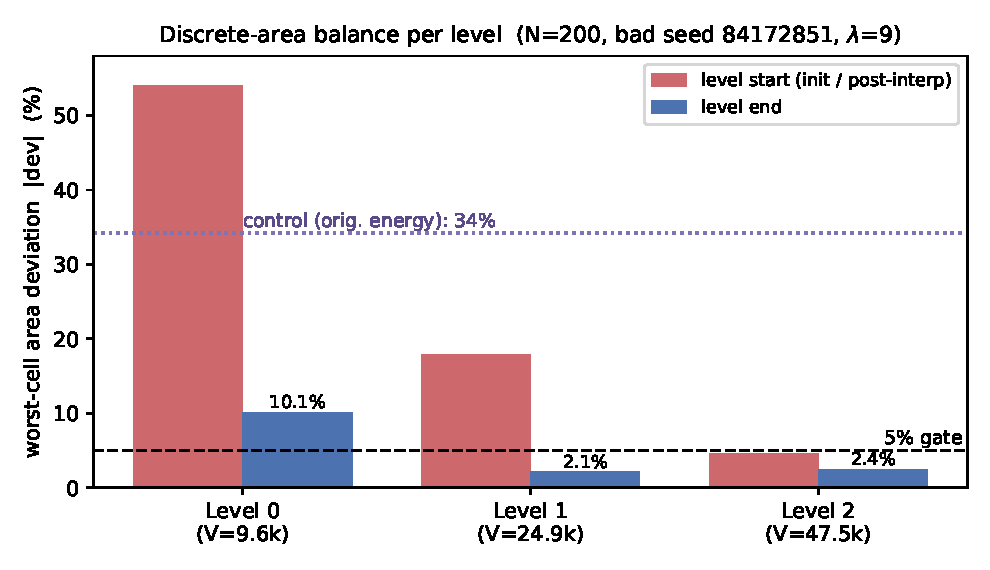
\includegraphics[width=0.82\linewidth]{fig_balance_by_level.pdf}
\caption{Worst-cell deviation at each level's start and end vs the control. The
mechanism clears the \(5\%\) gate; the control (dotted) stays at \(34\%\).}
\label{fig:levels}
\end{figure}

\section{Result 2 --- why no level triggered mesh refinement}
Both completed levels ran to the \(30{,}000\)-iteration cap; the log contains no
``Refinement triggered'' line. The cause is the trim, not a stuck optimizer. Every
\code{wta\_trim\_period}\,\(=200\) accepted iterations the trim retargets the per-cell
area target \(d\), re-projects, and re-baselines the energy --- each retarget bumps
\(E\) up before the next descent, so the energy \textbf{sawtooths and never plateaus}
(level-0 tail: \(E\) oscillates \(\approx409\text{--}437\), amplitude \(\sim8\)). The
refinement trigger fires on an energy plateau (\(\Delta E<10^{-8}\) held for 30
checks); the sawtooth's swings are nine orders of magnitude above that, so the
plateau criterion is structurally impossible to satisfy. This behaviour is
\emph{new}: no standard/production config sets any of the three territory flags
(verified), so previous N\(=\)100/150/200 runs plateaued cleanly and triggered
normally. The extra iterations are not wasted spinning --- the balance keeps
improving --- but the level cannot stop itself.

\section{Result 3 --- refinement is necessary, not merely faster}
The trajectory of the worst deviation \emph{within} each level
(Fig.~\ref{fig:traj}) settles the design question of whether one could simply run the
coarsest level longer:
\begin{itemize}
\item \textbf{Level 0 is floor-limited.} Its worst deviation flatlines at
  \(\approx10\%\) --- \emph{twice} the \(5\%\) gate --- with a tail rate of
  \(0.23\%/1000\) iterations (pure sawtooth noise). The count of bad cells keeps
  falling (\(14\to4\)), but the \emph{worst} cell is stuck, and the gate needs
  \emph{every} cell under \(5\%\). At 48 verts/cell the discretization cannot
  represent \(200\) equal areas below \(\approx10\%\); more iterations do not help.
\item \textbf{Level 1 crosses the gate, steeply.} At 124 verts/cell the achievable
  floor drops to \(\approx2\%\); the first \(5000\) iterations fall at
  \(2.2\%/1000\) (\(\sim10\times\) level 0's tail), reaching \(0\) imbalanced by
  \(\sim\)iter \(9000\).
\end{itemize}
The \(5\%\) gate lies \emph{between} the two levels' resolution floors
(\(f_b\propto1/\sqrt{V/N}\), the validity plan's band-fraction law), so refinement is
what crosses it. Note the gate was crossable at just \textbf{124 verts/cell} here ---
the validity plan's mesh-budget floor guessed \(\sim\)600 for margin, so
\(\sim\)250--300 finest may suffice (a 2--4\(\times\) compute rebate at N\(=\)1000,
worth confirming).

\begin{figure}[h]\centering
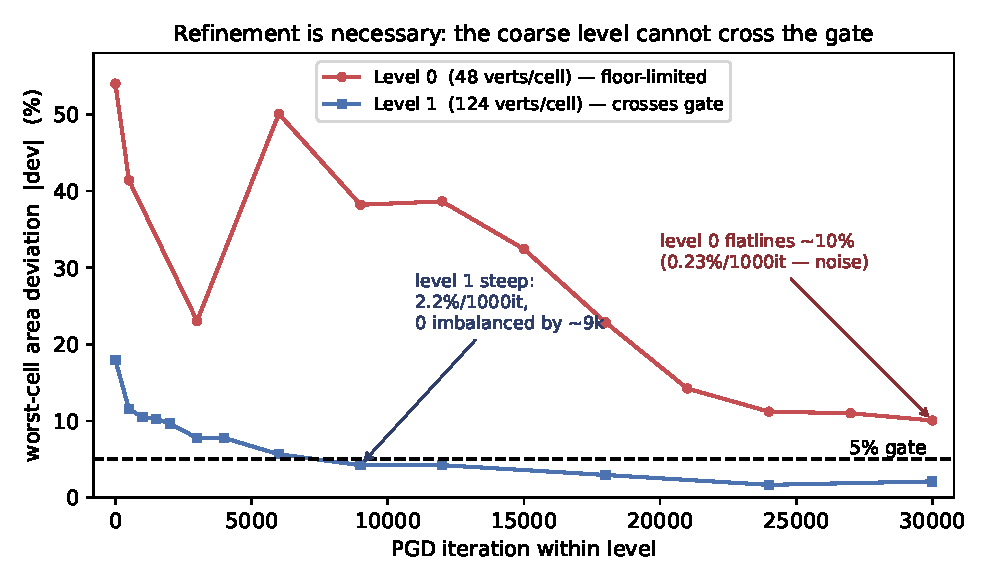
\includegraphics[width=0.82\linewidth]{fig_trajectory.pdf}
\caption{Worst-cell deviation vs iteration within levels 0 and 1. Level 0 floors
above the gate; level 1 (finer) descends \(\sim\!10\times\) faster and crosses it.}
\label{fig:traj}
\end{figure}

\section{Conclusions and implications}\label{sec:conclusions}
\emph{(Conclusion~1 is qualified by the addendum of \S\ref{sec:addendum}: it holds
for area, not for connectivity.)}
\begin{enumerate}
\item \textbf{The balance term works} on the hardest case (bad seed, \(\lambda\)
  immune) --- the anti-lottery property N\(=\)1000 requires. This confirms Stage~6.
\item \textbf{Its cost is diagnosed, not fundamental.} The slowness (level 0 alone
  \(9.5\)\,h, level 1 \(\sim31\)\,h, both to the cap) is the trim sawtooth preventing
  early triggering plus genuinely-continued optimization --- both tunable.
\item \textbf{The coarse-only schedule needs the switch \emph{after} level 1, gated on
  the imbalance metric, not fixed at level 0.} Level 0 cannot clear the gate (floor);
  the machinery must run until a level's floor drops below the gate (level 1 here),
  then the cheap original energy carries the already-balanced fine levels (level 2
  started at \(0\) imbalanced). Dropping the trim on the cheap levels also restores
  clean plateaus and normal triggering. See
  \codefile{docs/plans/PHASE1\_COARSE\_ONLY\_WTA\_SCHEDULE.md}.
\item \textbf{Refine on a balance/stationarity plateau, not raw energy.} Level 0's
  balance flatlined by \(\sim\)iter \(22\)k while the trim-masked energy kept crawling;
  a gate-aware trigger would have refined there, saving \(\sim\)3\,h at no cost to the
  result.
\end{enumerate}

% =====================================================================
\section{Addendum (2026-08-03) --- the connectivity regression and its
cost}\label{sec:addendum}
% =====================================================================

\begin{tcolorbox}[colback=gray!4!white, colframe=gray!50!black,
                  title={Provenance --- addendum}, fontupper=\small]
\begin{tabular}{@{}l@{\hspace{1.5em}}p{0.66\linewidth}@{}}
Date            & 2026-08-03 (analysis of the run of 2026-07-30\,\ldots\,08-03) \\[3pt]
Status          & \textbf{measured} (mid-ladder: level~2 checkpoint; the run never
                  reached its final level) \\[3pt]
Surface         & torus \(T(R{=}1.0,\ r{=}0.6)\), \(N{=}200\), seed \(61803399\),
                  \(\lambda{=}11\), 5 levels, \code{init\_method: seeded} \\[3pt]
Source run      & \textbf{territory:} \code{run\_20260730\_211516}, config
                  \codefile{parameters/torus\_200part\_coarse\_seeded\_s61803399\_lam11\_adaptive.yaml}
                  (\code{wta\_schedule: adaptive}, margin \(0.03\), re-arm \(0.05\)),
                  SLURM job \code{6371929} on UPPMAX Pelle, 4\,d wall.
                  \textbf{Control:} \code{run\_20260722\_175451} --- \emph{same}
                  seed, \emph{same} \(\lambda{=}11\), \emph{same} 5-level mesh,
                  machinery \textbf{OFF}: \(0\) dead / \(0\) imbalanced /
                  \(0\) fragmented, worst area deviation \(1.7\%\), run to
                  completion and finalised as a deliverable. \\[3pt]
Producing script& \codefile{testing/check\_fragmentation.py} (added for this
                  analysis) on \code{solution/checkpoint\_level02.h5};
                  \code{relaxation.log} for the timing and trim trace \\[3pt]
Anchor          & \code{n\_fragmented} \(=14\) with \code{n\_imbalanced} \(=1\)
                  and \code{dead} \(=0\) at level~2; worst cell \(198\), stray
                  \(43.57\%\) of target \\
\end{tabular}
\end{tcolorbox}

\subsection{Why this addendum exists}
The July report measured \emph{discrete-area imbalance} and found the balance term
fixes it. Connectivity was never tested. \S\,4b of
\codefile{docs/reference/winner\_take\_all\_partition\_gap.md} had by then recorded a
third failure mode --- \textbf{split cells}, whose winner-take-all territory holds
the right \emph{total} area in two or more disconnected islands --- and attributed
it to the seed lottery. This addendum tests that attribution, and finds it false.

\subsection{Result 4 --- the term fragments cells}
The reseed run used the seed \emph{proven clean} at this \(N\), \(\lambda\), and
mesh. Checked mid-ladder at \code{checkpoint\_level02.h5} (levels 0--1 complete,
\(V{=}24{,}948\), \code{wta\_active=True}):

\begin{center}\small
\begin{tabular}{@{}lrrr@{}}
\toprule
 & \textbf{control} & \textbf{seed 84172851} & \textbf{seed 61803399} \\
 & term OFF, final & term ON, final & term ON, level~2 \\
\midrule
dead cells        & 0            & 0            & 0 \\
imbalanced cells  & 0            & 0            & 1 \\
\textbf{fragmented cells} & \textbf{0} & \textbf{3} & \textbf{14} \\
worst stray       & ---          & 57\% (cell 58) & 43.6\% (cell 198) \\
most pieces       & ---          & 4            & 7 (cell 16) \\
\bottomrule
\end{tabular}
\end{center}

These are not threshold artifacts. Target area is
\(4\pi^2 R r/200 = 0.1184\); cell \(198\) holds
\(0.0663 + 0.0474 + 0.0042 = 0.1179\) --- on target, in three places, its second
piece \(40\%\) of a whole cell. Cell \(198\) does \emph{not} appear in the
imbalanced list. Only \(15\) cells have more than one raw component and \(14\)
clear the \(1\%\) significance threshold, so the filter is barely binding.

\paragraph{The control is matched.} \code{run\_20260722\_175451} differs from the
territory run \emph{only} in the machinery flags. It finished all five levels with
\(0\) fragmented cells and was finalised as a deliverable. The single remaining
mismatch is the comparison level (2 vs.\ final), and it cuts against the term: the
control was clean \emph{at the end}, while the territory run is already at \(14\)
\emph{mid-ladder}, with no mechanism that would heal it --- nothing in the energy,
the balance term, or the trim penalizes disconnection, so an area-balanced
fragmented cell is a stable fixed point.

\subsection{Result 5 --- the causal trace points at the trim}
\code{relaxation.log} records the trim's worst-deviation target at each retarget.
At level~0 it was dominated for hours by cell \(198\) (deviation \(41.8 \to 44.4
\to 53.1 \to 55.8 \to 57.8 \to 61.2 \to 67.0 \to 63.7\%\)) and cell \(16\)
(\(48.2, 45.4, 38.3, 37.0, 35.4\%\)), with cell \(37\) still flagged at the level
end. Those are precisely the \textbf{two worst fragmented cells} at level~2
(\(198\) at \(43.6\%\); \(16\) in seven pieces), and \(37\) is in the flagged list.
The trim drove their \emph{total} area to target by giving them disconnected
territory. It was also \textbf{clamp-saturated} --- \code{d range [0.800, 1.200]}
\(\times \bar A\), exactly \(\pm\)\code{wta\_trim\_clamp}\(=0.20\) --- for most of
the run, i.e.\ pushing at maximum authority.

Consistent with this, the \(3\)-fragment run \code{run\_20260722\_121925} saw its
fragment count \emph{fall} (\(8 \to 6 \to 3 \to 3\)) over exactly the levels that
had handed off to the cheap original energy. In the present run the adaptive
handoff \textbf{never fired} (level ends \(12.69\%\) and \(8.31\%\), both above
\code{wta\_switch\_margin}\(=0.03\)), so the trim ran on \emph{every} level.

\subsection{Result 6 --- the wall-clock cost}
No level ever triggered mesh refinement; every completed level ran to the
\(30{,}000\)-iteration cap. The \S\ref{sec:conclusions} conclusion~4 fix (refine on
a balance/stationarity plateau) was implemented and \emph{still} did not fire:
\(\norm{g_t}\) flatlined at \(\approx 20.33\), four orders above
\code{refine\_grad\_tol}\(=10^{-2}\), and the plateau fallback needs \(30\)
consecutive \(\abs{\Delta \norm{g_t}} < 10^{-4}\), which the trim's every-200-iteration
retarget breaks. Because the trim continuously moves the target, \(\norm{g_t}\) has
no reason to approach zero --- the balance-plateau trigger is structurally
unreachable while the trim runs.

\begin{center}\small
\begin{tabular}{@{}lrrrr@{}}
\toprule
Level & mesh & \(V\) & iterations & wall time \\
\midrule
1 & \(100\times96\)  & \(9{,}600\)  & 30{,}000 (cap) & \(11.2\)\,h \\
2 & \(162\times154\) & \(24{,}948\) & 30{,}000 (cap) & \(53.5\)\,h \\
3 & \(224\times212\) & \(47{,}488\) & \(9{,}500\) (killed) & \(31.4\)\,h \\
4 & \(286\times270\) & \(77{,}220\) & --- & --- \\
5 & \(348\times328\) & \(114{,}144\) & --- & --- \\
\bottomrule
\end{tabular}
\end{center}

Four days of wall clock bought \(2.4\) of \(5\) levels. At the observed
\(11.9\)\,s/iteration, level~3 alone needs \(\approx 99\)\,h; extrapolating the
measured scaling to levels 4--5 puts the full ladder at \(\approx 20\) days. The
job was killed without ever writing a final solution or \code{metadata.yaml}, so
none of the three validity gates ever ran --- the \(14\) fragments were found only
by checking the checkpoint directly.

\subsection{Interpretation}
At \(N{=}200\) the original energy already produces a valid, finalised partition
(the control). Against that baseline the territory-aware machinery is a
\textbf{net regression on two axes}: it makes the run roughly an order of magnitude
more expensive \emph{and} it converts area-deficient cells into area-correct
\emph{disconnected} ones, which are strictly worse for Phase~2 (a split cell yields
multi-loop contours the equal-area/Steiner machinery is not built for).

This does not retract Result~1. The term does what it was designed to do --- it
enforces \emph{total} discrete area, and on the bad seed it did so where \(\lambda\)
could not. The defect is that total area is the wrong invariant to enforce alone:
area and connectivity must be enforced together, or fixing the first breaks the
second. The motivating case for the term was \(N{=}300\), which the original energy
does not solve; the honest reading is that the term is \textbf{not yet ready} to be
the answer there either, because it would carry this fragmentation with it.

\paragraph{No figure.} The addendum's numbers come from a checkpoint that lives on
the cluster and is not in this repository, so \codefile{make\_figures.py} is
unchanged and no new \code{fig\_*.pdf} is generated. The measurement is reproducible
with \codefile{testing/check\_fragmentation.py} against that checkpoint.

\section{Caveats}
Single seed / single \(\lambda\) (by design --- the point is the \emph{bad} case).
The run was interrupted mid-level-2, so the formal finest-level completion gate was
not reached; a cluster re-run (with checkpoint/resume, and preferably the tuned
schedule of conclusion~3) is needed to close it. The next A/B is N\(=\)300 vs
\code{run\_20260714\_224821} (predicted \(9\to\le1\) over gate).

\paragraph{Addendum caveats (2026-08-03).} The connectivity comparison of
\S\ref{sec:addendum} is at level~2 for the territory run and at the final level for
both controls; there is no term-OFF measurement at level~2 specifically. The
decisive experiment is cheap and not yet run: relax seed \(61803399\),
\(\lambda{=}11\) to level~2 with \code{wta\_schedule: off} and count fragments.
Two seeds only. That the \emph{trim} rather than the \emph{balance term} is the
fragmenting component is an inference from the log trace and the handoff
correlation --- the two have never been enabled separately, and
\code{wta\_balance\_enabled} / \code{wta\_trim\_enabled} are independent flags, so
that A/B is also available.

\end{document}
